\documentclass[11pt]{article}
\usepackage{fullpage}
\usepackage{setspace}
\usepackage{amsmath}
\usepackage{fancyvrb}
\usepackage{enumerate}
\usepackage{pgfplots}
\usepackage{graphicx}
\usepackage{float}
\usepackage{multirow}
\usepackage[format=hang,labelsep=quad]{caption}
\usepackage{subfig}
\usepackage{array}
\usepackage{multirow}

\renewcommand\thesubfigure{\roman{subfigure}}


\begin{document}
\noindent\large{Math 5365}\\
\large{Data Mining 1}\\
\large{Homework 13}\\
\large{Mary Barker}
\doublespace
\begin{enumerate}
\item 
  Split wdbc.data into 70\% training and 30\% test data

  \begin{Verbatim}
  splitset <- splitdata(wdbc, 0.7, FALSE)
  train <- splitset$train
  \end{Verbatim}
\begin{enumerate}
\item \label{i:pt1}
 Fit a neural network with size=1 to the training data, plot it, 
 and calculate the accuracy and area under the ROC curve using the 
 test data.

The accuracy for this neural network was 84.79532\%.
\begin{center}
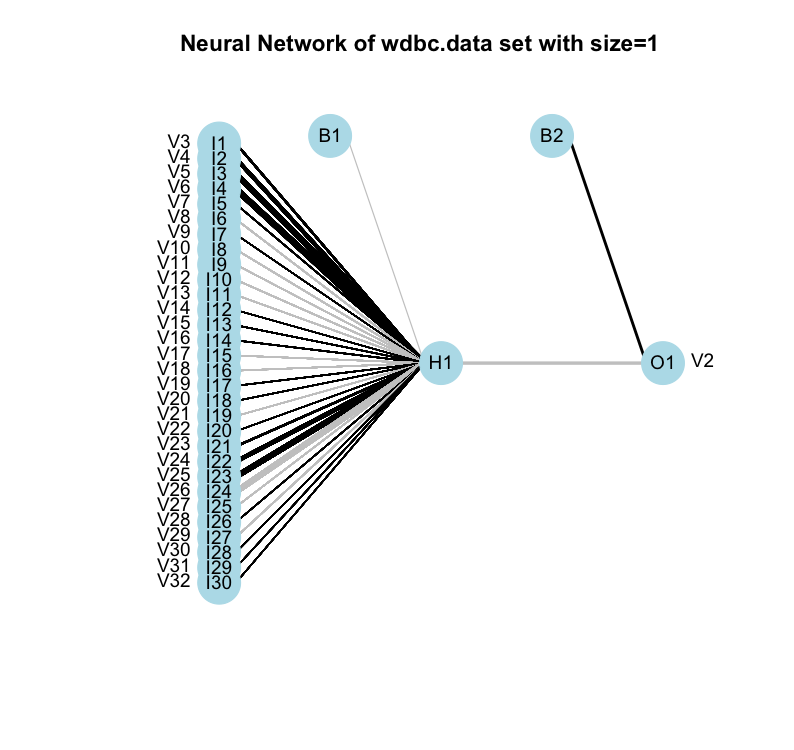
\includegraphics[scale=0.35]{nnet_1}
\end{center}
\begin{center}
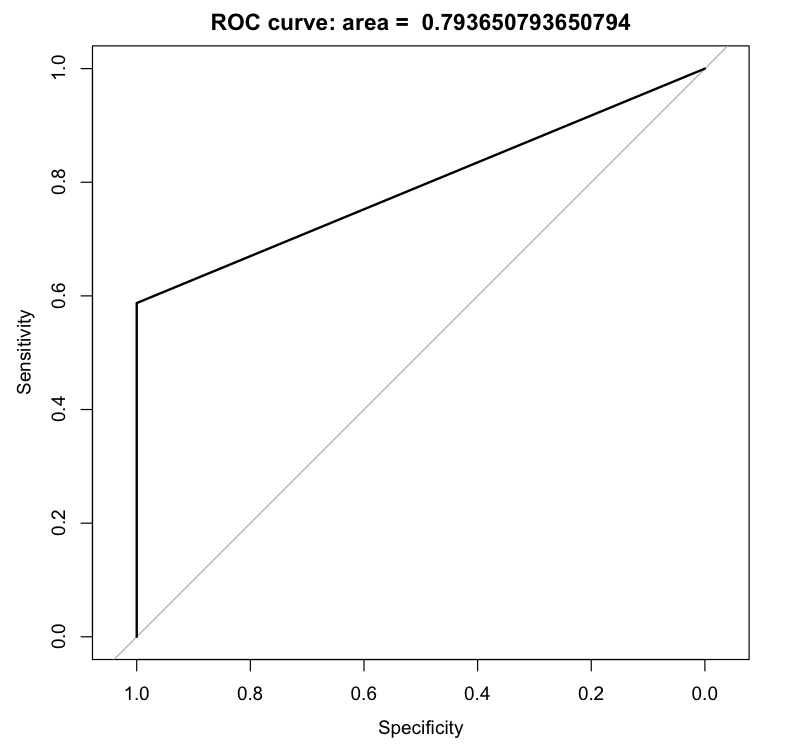
\includegraphics[scale=0.35]{roc_curve_1}
\end{center}

\item Use 10-fold Cross-validation to find the optimal value of size

  \begin{Verbatim}
  error <- rep(-1, 29)
  
  for(s in 2:30){
    error[s - 1] <- kfold_val(k = 10, 4, wdbc = wdbc, idx = 1, val=s)$error
  }
  
  s <- which.max(1 - error)
  1 - error[s]
  
  \end{Verbatim}
\item Repeat part \ref{i:pt1} for the optimal value of size.
The accuracy using the optimal size parameter is 90.64327\%.

\begin{center}
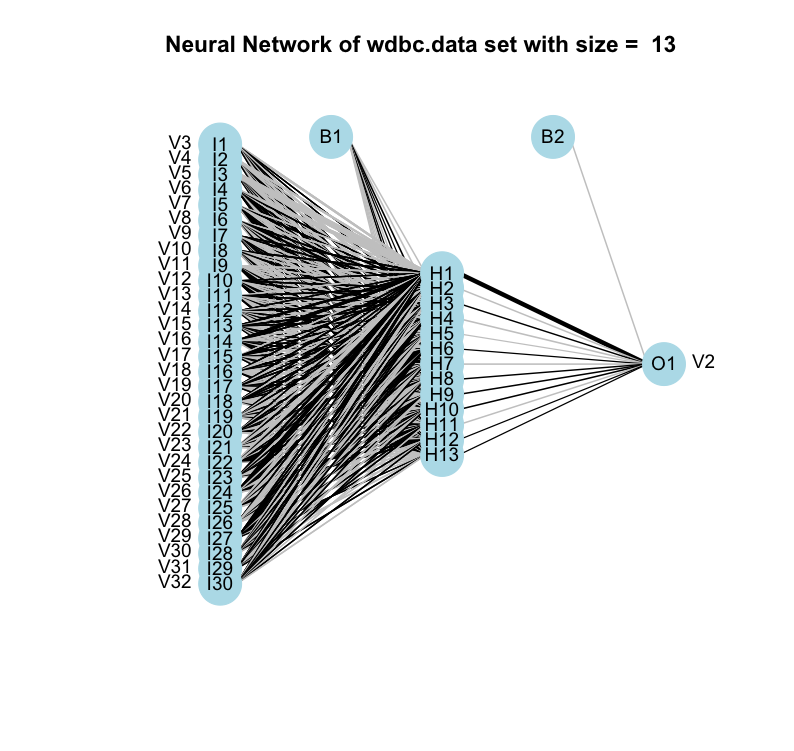
\includegraphics[scale=0.35]{nnet_13}
\end{center}
\begin{center}
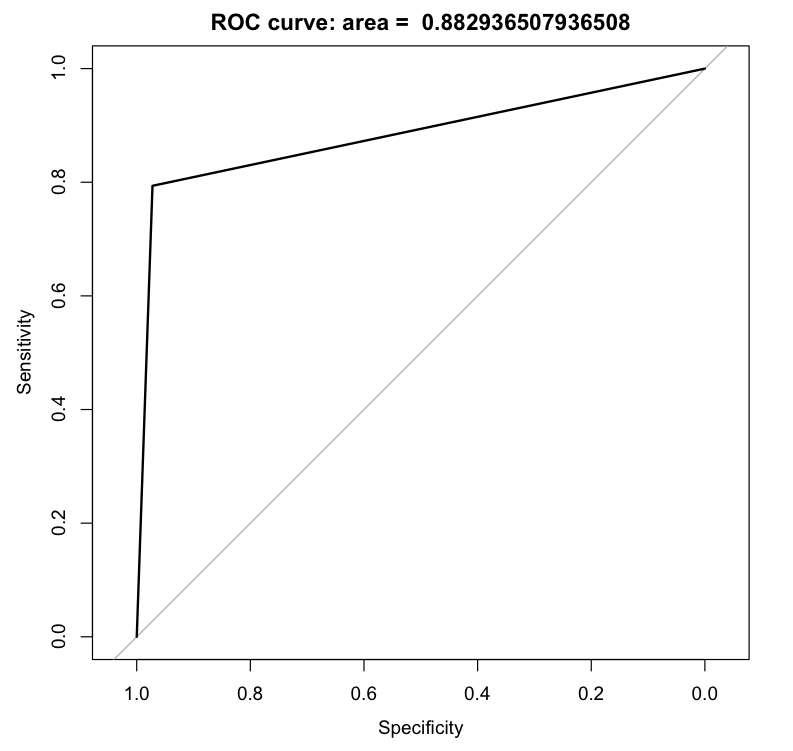
\includegraphics[scale=0.35]{roc_curve_13}
\end{center}

\end{enumerate}
\item 
\begin{enumerate}
\item Randomly generate 100 points from $[0, 2\pi]$, and fit a neural network 
for predicting $y = sin(x)$ using this data. 

\begin{Verbatim}
x <- runif(100, 0, 2 * pi)
y <- sin(x)
dset <- data.frame(y = y, x = x)
sinmodel <- nnet(y~x,size = 10, linout=TRUE)
\end{Verbatim}

\item
 Use 10-fold cross validation to find the optimal value of size for 
 this neural network. 

\begin{Verbatim}
len = 30
n_error = rep(-1, len - 1)
for(s in 2:len){
  n_error[s - 1] <- kfold_val(10, 5, dset, 1, s)$error
}
which.max(1 - n_error)
s <- s + 1
model <- nnet(y~x,size=s,linout=TRUE)
predsin <- predict(model,dset)
\end{Verbatim}

\item
 Plot $y = sin(x)$ and the predictions from your neural network on the 
 same graph. 

\begin{center}
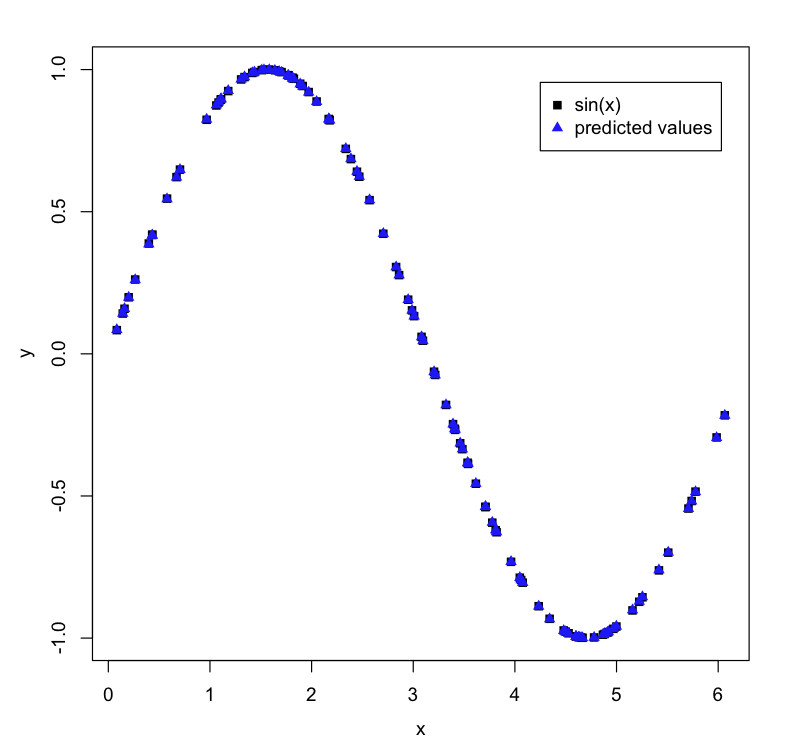
\includegraphics[scale=0.35]{sinvs_computed}
\end{center}

\end{enumerate}

\end{enumerate}

\newpage
\begin{Verbatim}
#Data Mining hw 13
library(nnet)
library(pROC)

wdbc <- read.table("~/Dropbox/Tarleton/data_mining/dfiles/wdbc.data", 
        header = FALSE, sep = ",")
wdbc <- wdbc[,-1]

# 1 Split wdbc.data into 70% training and 30% test data

splitset <- splitdata(wdbc, 0.7, FALSE)
train <- splitset$train

#a Fit a neural network with size=1 to the training data, plot it, 
#  and calculate the accuracy and area under the ROC curve using the 
#  test data.

model <- nnet(V2~., wdbc[train,], size = 1, linout=FALSE)
#summary(model)
predV2 <- predict(model, newdata=wdbc[-train,], type='class')
confmatrix(wdbc$V2[-train], predV2)
plot(model, main='Neural Network of wdbc.data set with size=1')

phat <- predict(model,newdata=wdbc[-train,],type='raw')[,1]
idx <- as.numeric(1 * (wdbc$V2[-train] == 'M'))
roc_curve <- roc(idx, phat)
title=paste('ROC curve: area = ', roc_curve$auc)
plot(roc_curve, main=title)

# b Use 10-fold Cross-validation to find the optimal value of size
error <- rep(-1, 29)

for(s in 2:30){
  error[s - 1] <- kfold_val(k = 10, 4, wdbc = wdbc, idx = 1, val=s)$error
}

s <- which.max(1 - error)
1 - error[s]

newmodel <- nnet(V2~., wdbc[train,], size = s + 1, linout=FALSE)
#summary(newmodel)
newpredV2 <- predict(newmodel, newdata=wdbc[-train,], type='class')
confmatrix(wdbc$V2[-train], newpredV2)
title=paste('Neural Network of wdbc.data set with size = ',s + 1)
plot(newmodel, main=title) 

phat <- predict(newmodel,newdata=wdbc[-train,],type='raw')[,1]
idx <- as.numeric(1 * (wdbc$V2[-train] == 'M'))
roc_curve <- roc(idx, phat)
title=paste('ROC curve: area = ', roc_curve$auc)
plot(roc_curve, main=title)
\end{Verbatim}

\end{document}
